\documentclass[a4paper,10pt]{article}
\usepackage[T2A]{fontenc}
\usepackage[utf8x]{inputenc}
\usepackage{ucs}
\usepackage{cmap}
\usepackage[english,russian]{babel}
\usepackage{amsmath}
\usepackage{color,graphicx}
\usepackage{indentfirst}
\usepackage{ucs} 
\usepackage[utf8x]{inputenc}
\usepackage{caption}
\usepackage{placeins}
\usepackage{amssymb}

\title{Обзор спайковых сетей}
\author{Чернышев Алексей}
\setlength{\parindent}{1cm}
\def\la{\left\langle\rule{0pt}{3em}}
\def\ra{\right\rangle}
\newcommand{\HRule}{\rule{\linewidth}{0.5mm}}



\begin{document}
\begin{titlepage}
\begin{center}
% Title
\HRule \\[0.4cm]
{ \huge \bfseries Cпайковые нейронные сети \\[0.4cm] }

\HRule \\[1.5cm]
% Author and supervisor
\begin{minipage}{0.4\textwidth}
\begin{flushleft} \large
\emph{Автор:}\\
асп. Чернышев Алексей
\end{flushleft}
\end{minipage}
\begin{minipage}{0.4\textwidth}
\begin{flushright} \large
\emph{Научный руководитель:} \\
д.ф.-т.н. Карпенко А.П.
\end{flushright}
\end{minipage}

\vfill

% Bottom of the page
{\large Август 2014}

\end{center}
\end{titlepage}


\tableofcontents
\clearpage
\section{Введение}
\indent Нейронные сети, как попытка воссоздать процессы интеллектуальной информационной обработки, так как это происходит в коре головного мозга, являются предметом исследования учёных больше полувека. Наработанные знания в этой сфере образовали такую область научных исследований, как нейроинформатика и теоретическая нейронаука.\\
\indent Первый взрыв интереса к нейронным сетям был подпитан гипотезой об устройстве мыслительного процесса аналогично машине фон-Неймана, когда каждый нейрон представлялся элементарной логической функцией из элементарной логики, и соединение таких нейронов в сети формировало сложную иерархическую логическую функцию. Именно в это время получили своё начало модели подобные нейрону Маккалола-Питтса (1943), которые являются до сих пор наиболее популярным решением, которое предлагает теория нейронных сетей.\\
\indent Однако, начиная с 1943, исследования процессов мышления и нейронов, как биологических элементов, значительно продвинулись, в особенности с появлением функциональной томографии и микроэлектродов в последние 20 лет. Таким образом, сегодня, нейроинформатика находится под влиянием переосмысления новых открытых качеств нейронов\cite{BohteReview}, как информационных вычислительных элементов.\\
\indent Спайковые нейронные сети являются той подобластью нейронного моделирования, которая концентрирует своё внимание на биологических деталях с целью поиска новых перспектив в изучении нейронных процессов.\\
\indent В данном обзоре рассматриваются спайковые модели нейронов, нейронных сетей и алгоритмов их обучения, которые в той или иной степени приближены к биологическому правдоподобию. Рассматриваются примеры использования таких сетей, как целью теоретических исследований, так и с целью прикладных применений.\\
\section{Биологическая основа нейронов}
\indent Человеческий мозг содержит в себе огромное количество соединенных между собой нейронов, нервных клеток, которые стали предметом интереса во многих областях, таких как нейрофизиология, теоретическая нейронаука, искусственный интеллект.\\
\indent Нейрон по своему строению довольно схож с другими клетками: тело нейрона окружено плазматической мембраной, внутри которой находятся ядро, цитоплазма и другие составляющие клетки. Однако, нейрон несет в себе особую функцию: нейрон выполняет приём сигналов от других нейронов, преобразует и передает их на вход другим нейронам или клеткам. Сигнал представляет из себя импульсы нервной активности, имеющих электрохимическую природу\\
\indent Нейроны крайне разнообразны по форме и нюансам функционирования, хотя существует возможность вывести наиболее типичную форму нейрона. На рис. \ref{bio_pic} отображена схема биологического нейрона. \\
\begin{figure}[ht]
\centering
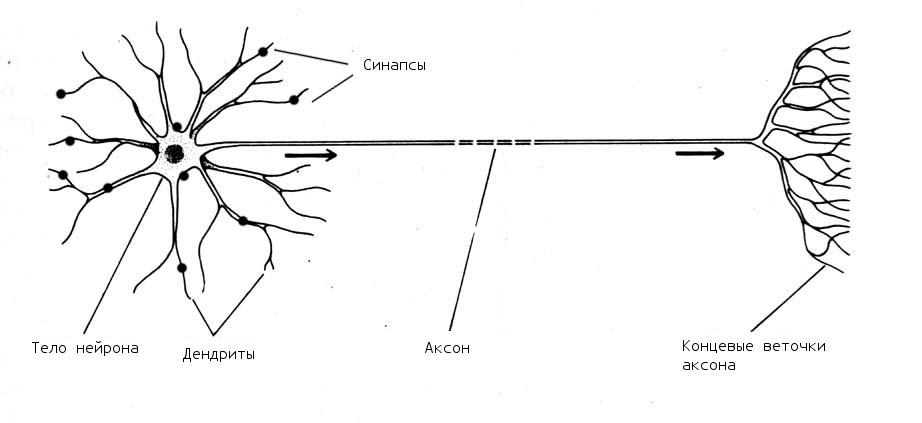
\includegraphics[width=1\linewidth]{bio_neuron.jpg}
\caption{биологический нейрон}
\label{bio_pic}
\end{figure}
\indent Прием нервных импульсов от других нейронов происходит посредством дендритов, на которых расположены синапсы - точки соединения нейронов между собой. Дендриты проводят входные импульсы с синапсов доставляя их клетке нейрона, которые специфичным образом возбуждают клеточную мембрану.\\
\indent Элетрохимические процессы внутри клетки делают нейрон в той или иной мере чувствительным к возбужденям мембраны, и когда возбуждение достигает определенного порога, потенциал на мембране на короткое время (около 2 мс) осуществляет резкий скачок вверх, порождая короткий импульс называемый спайком. Аксон является проводником таких импульсов к другим клеткам. После выработки спайка нейрон переживает т.н. рефракторный период, в течении которого чувствительность мембраны к возбуждениям резко спадает.\\
\indent Синапсы, при более подробном взгляде, представляют из себя не менее сложный механизм, чем сам нейрон. Типичный синапс, как контакт между двумя нейронами, представляет собой пузырек наполненный нейромедиаторами находящийся на аксоне пресинапатической клетки и мембрана чувствительная к нейромедиаторам на дендрите постсинаптической клетки. При возбуждении аксона нейромедиаторы синапса начинают освобождаться в пространство между пресинаптической и постсинаптической мембраной - синаптическую щель (10-50 нм), где они встречаются с чувствительными белками на постсинаптической мембране. Следствием такой структуры является односторонее проведение нервного импульса. Количество высвобожденного и принятого нейромедиатора варьируется, и ``натренированный'' синапс, будет проводить гораздо большее количество импульса засчёт большего количества нейромедиаторов в синаптическом пузырьке и рецепторов на постсинаптической мембране. В нейроинформатике, обычно, пренебрегают такими тонкими деталями, и вводят ``веc'' синапса, который характеризует насколько эффективно синапс может проводить импульс.\\
\indent Ещё один феномен касающийся нюансов функционирования биологического нейрона - сенсорная адаптация\cite{Phizi}. Нейрон при получении импульсов с одной и той же характеристикой, как правило, начинает ``привыкать'' и приспосабливаться, чтобы тратить меньше энергии при интеграции этого сигнала. Как следствие, интенсивность его ответа угасает. Исследователями в области теоретической нейронауки этот феномен довольно пристально исследуется и существуют выводы об оптимальности такого поведения, с точки зрения оптимизации переданной информации нейроном \cite{Adapt,TripleAdapt}.

\subsection{Модель Ходжкина-Хаксли}
	В 1952 году Алан Ллойд Ходжкин и Эндрю Хаксли разработали первую, наиболее подробную на тот момент математическую модель нейрона. Модель была построена на основе динамики генерации и передачи нервного сигнала в гигантcком аксоне кальмара.\\
	\indent Данную модель сложно применить в решении реальных задач, которые решает нейроинформатика, так как её моделирование ресурсоёмко - около 1200 операций с плавающей точкой для моделирования одной милисекунды\cite{BohteReview}. Однако, модель играет важную научную и историческую роль в нейронауках.\\
	\indent Общая динамика потенциала нейрона описывается плавным затуханием значения потенциала на мембране $u_{m}(t)$, со скоростью, которая характеризуется ёмкостью мембраны $C_{m}$
	\begin{equation}\label{eq:hh}
	C_{m}\frac{du_{m}(t)}{dt}+I_{ion}(t)=I_{ext}(t).
	\end{equation}	 
	\indent Здесь $I_{ion}(t)$ - сумма ионных токов внутри клетки, $I_{ext}(t)$ - приложенный ток снаружи клетки.\\
	\indent Сложность уравнения \eqref{eq:hh_ion}	 таится в моделировании ионных токов для каждого типа ионов. В модели Ходжкина-Хаксли динамика ионных токов характеризуется наличием т.н. ионных каналов, открытие или закрытие которых влияет на общую динамику напряжения на мембране. В исходной модели Ходжкина-Хаксли было два вида ионов $Na^{+}$ и $K^{-}$, где ионный поток $Na^{+}$ описывается тремя каналами вероятность открытия которых $p_{m}$ и одним каналом с вероятностью открытия $p_{h}$, ионный поток $K^{-}$ описывается четырьмя каналами с вероятностью открытия $p_{n}$\cite{Genesis}.\\ 
	\indent Динамика вероятности открытия-закрытия каналов, выражается дифференциальным уравнением первого порядка
	\begin{equation}\label{eq:hh_pch}
	\frac{dp_{i}(t)}{dt} = \alpha_{i}(u_{m}(t))(1-p_{i}(t)) - \beta_{i}(u_{m}(t))p_{i}(t),
	\end{equation}	 
	где $\alpha_{i}(u_{m}(t)), \beta_{i}(u_{m}(t))$ константы зависящие от потенциала на мембране, которые характеризуют скорость закрытия и открытия канала, соответственно. Временной промежуток, спустя который вероятность достигает равновесия, описывается константой
	\begin{equation}\label{eq:hh_t}
	\tau_{i}=\frac{1}{\alpha_{i}(u_{m}(t))+\beta_{i}(u_{m}(t))}.	
	\end{equation}
	\indent Таким образом динамику ионных токов для модели Ходжкина-Хаксли, можно описать уравнением
	\begin{align}\label{eq:hh_ion}
	I_{ion}(t) &= \begin{aligned}[t]
	&\bar{g}_{Na}\;p_{m}^{\;3}(t)\;p_{h}(t)\;(u_{m}(t)-E_{Na}) +	\\
	+\;&\bar{g}_{K}\;p_{n}^{\;4}(t)\;(u_{m}(t)-E_{K})+\bar{g}_{L}(u_{m}(t)-E_{L}),	\\
	\end{aligned}	
	\end{align}
	где $p_{m}(t), p_{h}(t), p_{n}(t)$ - вероятности открытия каналов, описываются уравнением динамики \eqref{eq:hh_pch}, которые включают соответствующие константы. Смысл и значения констант можно найти в оригинальной работе\cite{HH}.\\
	\indent Не смотря на то что применение такой модели в задачах машинного обучения затруднительно, данная модель хорошо отражает особенности динамики нейрона.

\section{Модели нейронов}
\subsection{Классические ИНС}
\subsubsection{Нейрон МакКалока-Питтса}
   Первая модель нейрона, положившая начало нейроинформатике  - модель МакКаллока-Питтса. Эта модель прочно заложила фундамент теории нейронных сетей, и исследования новых свойств этой модели не   прекращаются по сей день.\\
   \indent Ключевой особенностью данной модели является то, что нейрон представляется, как взвешенный сумматор входных скалярных признаков $\boldsymbol{x}=(x_{1},x_{2},...,x_{n})$. Обработка нейроном входов происходит пропусканием взвешенной суммы через нелинейную функцию $\phi(x)$, называемую функцией активации\\
   \begin{equation}\label{eq:sum_mp}
   y(x) = \phi(\sum_{j=1}^{n}w_{j}x_{j}).
   \end{equation}
\indent Здесь $\boldsymbol{w}=(w_{1}, w_{2},...,w_{n})$ выражает вектор весов взвешенного сумматора (синапсов нейрона), $y(x)$ - скалярная величина, которая выражает результат обработки нейроном вектора $\boldsymbol{x}$.\\	
	\indent В качестве нейлинейной функции, наиболее популярным выбором является сигмоидальная функция\cite{Zaencev1999}. Данная функция удобна своей непрерывностью и гладкостью, и позволяет ограничить выход нейрона  отрезком значений $y(x)\in[0,1]$, такой выход можно интерпретировать как уровень активации нейрона, в зависимости от входного вектора $\boldsymbol{x}$ и настройки весов $\boldsymbol{w}$, что имеет свою, пускай и отдаленную, биологическую подоплёку. \\
   \indent Не смотря на ошеломляющий успех и широкое применения данной модели  и производных моделей в прикладных задачах, с биологической точки зрения такие нейроны, только отдаленно напоминают, то как работают настоящие нейроны в мозгу.\\
   \indent Важным отличием такого нейрона от биологического является тот факт, что данная модель не имеет внутреннего состояния и не может быть представлена в виде динамической системы\cite{Zaencev1999}. Данное свойство серьезно ограничивает круг задач в которых можно было бы применить нейронные сети. 
\subsubsection{Радиальные нейронные сети}
\indent Метод радиальных базисных функций исторически возник на базе сочетания теории приближений и нейронных сетей. В качестве элементарного элемента для построения таких сетей служит аппроксимирующая функция - нейрон, и  линейная комбинация результатов активации $N$ нейронов приближает значение целевой функции $y(\boldsymbol{x}), x\in \mathbb{R}^n$
   \begin{equation}\label{eq:rbf}
   y(\boldsymbol{x}) = \sum_{i=1}^{N}w_{i}\phi(|\boldsymbol{x}-C_{i}|).
   \end{equation}
\indent Задача обучения таких сетей состоит в подборе таких параметров $C_{i},w_{i}$ для $i\in \{1,N\}$, чтобы уравнение \eqref{eq:rbf} удовлетворялось хотя бы приближённо. Если предположить, что все $C_{i}$ известны и аппроксимирующая функия $\phi$ выбрана, то решение такой задачи сводится к решению системы линейных алгебраических уравнений. \\
\subsection{Спайковые модели}   
\indent Нейронные модели описанные в данной секции принадлежат к семейству спайковых моделей. Простота этих моделей позволяет перейти от анализа одного-двух нейронов к анализу популяций нейронов соединённых в сети, опуская биологическую точность, но сохраняя общие черты характерные для биологических нейронов.\\
\subsubsection{Модель Integrate-and-Fire}

\indent Модель Integrate-and-fire имеет большую историю. Ещё в 1907 году 	французский физиолог Луи Лапик эксперементируя с лягушками описал модель возбуждения нервных клеток используя RC-цепь\cite{Lapicque}. За свою вековую историю модель, благодаря своей простоте и, главное, биологической оправданности, получила много применений.\\
   \indent Динамика модели описывается динамической системой с одной переменной, довольно похожей на уравнение \eqref{eq:hh}, за тем исключением, что ионные токи не моделируются, а спайк генерируется нейроном при достижении заранее заданного порога:\\
   \begin{equation}\label{eq:iaf}
   \tau_{m}\frac{du}{dt} =-u+R I(t),
   \end{equation}
при $u \geq \vartheta$ потенциал мембраны сбрасывается   
   \begin{equation}\label{eq:iaf_reset}
   u \leftarrow u_{r},
   \end{equation}
где $\vartheta$ - порог напряжения, временная константа мембраны $\tau_{m}=RC$, $R$ и $C$ - сопротивление и ёмкость RC-цепи соответственно, $I(t)$ - приложенный ток извне, $u_{r}$ - константа описывающая потенциал мембраны покоя нейрона.\\   
\indent Данная нейронная модель подходит для конструирования нейронных сетей: приложенный ток $I(t)$ можно рассмотреть, как ток, получаемый нейроном через синапсы от других нейронов. Допустим нейрон соединён с N входными спайковыми нейронами через синапсы с определенными весами, тогда приложенный ток описывает равенство
\begin{equation}\label{eq:iaf_syn}
I(t) = \sum_{j=1}^{N} w_{j}\; \epsilon(t-t_{j}^{f}),
\end{equation}
где $\epsilon(t)$ - низкочастотный фильтр, как правило, в виде затухающей экспоненты, который характеризует спайк на синапсе, такая функция хорошо описывает импульс переданный в процессе передачи нейромедиаторов, $w_{j}$ - скаляр выражающий вес на синапсе, $t_{j}^{f}$ - время спайка на входном нейроне.\\

\subsubsection{Модель Ижикевича}
\indent Данная модель является наиболее популярным компромиссом между вычисляемой сложностью модели и её биоподобности. Динамическая система с двумя переменными и квадратичной зависимостью при хорошем подборе коэффициентов уравнения может воспроизводить большинство известных нейронных паттернов\cite{IzhSimpleModel}, включая, например, такие сложные как, высокочастотные спайки (fast spiking) или взрывной поток спайковых импульсов (bursting).\\
\indent Модель описывается системой уравнений
\begin{equation}\label{eq:izh}
\left\{  \begin{array}{c} \begin{aligned}
	\frac{du}{dt} &= 0,04u^2+5u+140-r, \nonumber \\
	\frac{dr}{dt} &= a(bu-r), \nonumber 
	\end{aligned}	
	\end{array} \right.
\end{equation}
при $v \geq \vartheta$ переменные сбрасываются:
\begin{equation}\label{eq:izh_reset}
\left\{  \begin{array}{c} \begin{aligned}
	u &\leftarrow c \nonumber, \\
	r &\leftarrow r+d,
	\end{aligned}	
	\end{array} \right.
\end{equation}
где $u, r$ - переменные динамической системы, $a, b, c, d, \vartheta$ - константы. Здесь $u$ отвечает за потенциал мембраны, $r$ - переменная отвечающая за восстановление нейрона. Преодоления порога описываемой константой $\vartheta$ и сброс переменных влечет за собой выработку нейроном спайка, который в данной модели является обычным событием, которое характеризуется временем, когда оно произошло.\\
\indent Пониженная вычисляемая сложность делает эту модель наиболее подходящей для масштабных и правдоподобных симуляций головного мозга, автором этой модели была проделана работа \cite{IzhTalam} по симуляции 3x3 см$^2$ таламо-кортикальной системы млекопитающего включающую $10^{11}$ нейронов и $10^{15}$ синапсов.
\subsubsection{Spike Response Model}
\indent Отдельным рядом стоит модель Spike Response Model. В своём оригинальном виде модель повторяет динамику модели Integrate-and-fire и, по сути, является его приближенным решением.\\ 
\indent Генерация спайков происходит таким же образом: при преодолении заданного порога, нейрон генерирует спайк. Однако, когда Integrate-and-fire представляется в виде дифференциального уравнения, SRM представляется в виде функции от времени $f(t)$ и совокупности фильтров:
\begin{equation}\label{eq:srm}
u(t) = u_{rest} + \sum_{j=1}^N w_{j} \sum_{t^{f}_{j}} \epsilon_{j}(t-t^{f}_{j}) + \sum_{t^{f}_{i}}\eta(t-t^{f}_{i}),
\end{equation}
здесь $u_{rest}$ - константа описывающая потенциал покоя, второе слагаемое представляет из себя интеграцию спайков с синапсов. Вторая сумма в этом выражении происходит по всем временам спайков $t^{f}_{j}$ на синапсе $j$. Для каждого времени спайка при помощи низкочастного фильтра $\epsilon$ измеряется вклад данного спайка в потенциал на синапсе $j$ в текущий момент времени $t$. Полученный потенциал синапса, модулируемый его весом $w_{j}$, суммируется по всем синапсам нейрона. Третье слагаемое является фильтрацией всех спайков нейрона функцией, которая описывает поведение нейрона после спайка, такая функция позволяет спайкам в прошлом повлиять на текущее состояние мембраны $u(t)$. Как правило, этой функцией описывается состояние рефрактерности нейрона.\\
\indent Тот факт, что эта модель является функцией от времени, позволяет напрямую выразить плотность вероятности спайков, пропустив напряжение на мембране через любую монотонно возрастающую функцию. Удобнее всего использовать экспоненциальный вид функции, иногда её модифицируют так, чтобы около определенного порогового значения мембраны вероятность генерации спайка резко возрастала. Выражение плотности вероятности позволяет описать процесс негомогенным пуассоновским процессом, что открывает широкие возможности для теоретического исследования спайкового нейрона.\\
\indent Добавление новых динамических свойств в Spike Response Model реализуется добавлением соотвествующих фильтров в уравнение \cite{AdaptThesis} либо модифицируя функцию плотности вероятности\cite{TripleAdapt}. 

\section{Обучение нейронных сетей}
\subsection{Обучение классических ИНС}
\indent Наиболее устоявшийся метод обучения нейронных сетей является метод обратного распространения ошибки. Нейрон Маккалока-Питтса, имея в основе дифференируемую на множестве натуральных чисел функцию активации, прекрасно подходит для оптимизации весов нейрона, для задания необходимого выходного сигнала.\\  
\indent Метод обратного распространения ошибки решает задачу оптимизации весов нейронов всей сети в зависимости от функции оценки, которая количественно отражает, то насколько выход сети решает поставленную задачу. В качестве примера возьмём квадрат отклонения выхода нейрона последнего слоя сети от целевого значения
\begin{equation}
E = \frac{1}{2}(t-y)^2,
\end{equation} 
где $E$ - ошибка нейрона, $t$ - целевое значение выхода нейрона, $y$ - выход нейрона.\\
\indent Имея для нейрона $j$ с $n$ синапсами выход равный
\begin{equation}
o_{j}=\phi (net_{j}) = \phi \left(\sum_{k=1}^{n}w_{kj}x_{k}\right),
\end{equation}
где функция активации $\phi(z)$ нелинейная и дифференцируема, например
\begin{equation}\label{eq:logist}
\phi(z)=\frac{1}{1+\exp^{-z}},
\end{equation}
можно взять частную производную функции оценки по весам можно выразить через цепочку производных
\begin{equation}\label{eq:bp_chains}
\frac{\partial E}{\partial w_{ij}} = \frac{\partial E}{\partial o_{j}} \frac{{\partial o_{j}}}{\partial net_{j}} \frac{{\partial net_{j}}}{\partial w_{ij}},
\end{equation}
где последний член \eqref{eq:bp_chains} правой стороны выражается
\begin{equation}
\frac{{\partial net_{j}}}{\partial w_{ij}} = \frac{\partial}{\partial w_{ij}} \left(\sum_{k=1}^{n}w_{kj}x_{k}\right) = x_{i}.
\end{equation}
\indent Частная производная выхода нейрона $j$ относительно его входа это частная производная функции активации. Например для логистической функции \eqref{eq:logist} получаем
\begin{equation}
\frac{{\partial o_{j}}}{\partial net_{j}} = \frac{\partial}{\partial net_{j}} \phi(net_{j}) = \phi(net_{j})(1-\phi(net_{j})).
\end{equation}
\indent Первый член \eqref{eq:bp_chains} правой стороны выражается просто в случае, если нейрон из выходного слоя
\begin{equation}
\frac{\partial E}{\partial o_{j}} = \frac{\partial E}{\partial y} = \frac{\partial}{\partial o_{j}} \frac{1}{2} (t-y)^2 = y - t  .
\end{equation}
\indent В случае когда нейрон $j$ из внутреннего слоя вычисления немногим усложняются. Рассмотрим функцию $E$ как функцию от $m$ входов нейронов предшествующего слоя
\begin{equation}
\frac{\partial E(o_{j})}{\partial o_{j}} = \frac{E(net_{1}, net_{2},...,net_{m})}{\partial o_{j}}.
\end{equation}
\indent Если взять полную производную по параметру $o_{j}$ рекурсивное выражение получает вид
\begin{equation}
\frac{\partial E}{\partial o_{j}} = \sum_{l\in L}\left(\frac{\partial E}{\partial net_{l}} \frac{\partial net_{l}}{\partial o_{j}}\right).
\end{equation}
\indent Собирая все выкладки вместе получаем
\begin{equation}\label{eq:bp_update}
\frac{\partial E}{\partial w_{ij}} = \delta_{j} x_{i},
\end{equation}
где
\begin{equation}
\begin{split}
\delta_{j} &= \frac{\partial E}{\partial o_{j}} \frac{\partial o_{j}}{\partial net_{j}} = \\ &=\begin{cases} (o_{j}-t_{j}) \phi(net_{j})(1-\phi(net_{j})), & \mbox{если }j\mbox{ выходной нейрон} \\ (\sum_{k}\delta_{j}w_{jk})\phi(net_{j})(1-\phi(net_{j})), & \mbox{если }j\mbox{ нейрон сети.} \end{cases}
\end{split}
\end{equation}
\indent Обновление весов можно осуществлять вычитая из $w_{ij}$ значение \eqref{eq:bp_update} помноженного на небольшой коэффициент обучения, осуществляя тем самым минимизацию функции ошибки методом градиентного спуска.
\subsection{Обучение спайковых нейронных сетей}
\subsubsection{Классическое правило Хэбба}
\indent Вопрос, как настоящий синапс обучается, стоит до сих пор, хотя огромное количество деталей этого процесса было открыто за последние полвека. Канадский физиолог Дональд Хэбб, ещё в 1949 году без возможности на тот момент проверить гипотезу заявил:\\
\indent ``Когда аксон нейрона А достаточно близок к тому чтобы возбудить нейрон Б и неоднократно или постоянно участвует в его активности, некоторые процессы роста или метаболических изменений имеют место в первой или обоих клетках, так, что эффективность возбуждения клеткой А клетку Б возрастает''\cite{Hebb1949}.\\
\indent Сейчас, когда современные технологии позволяют более серьезно изучить вопрос, можно сказать, что заявляение Хэбба было недалеко от истины. Было поставлено большое количество экспериментов (см. обзор \cite{BiPoo}) для выявления зависимости между изменением веса синапса и активности синапса и нейрона, которые породили множество, как феноменологических, так и теоретических моделей.\\
\indent На сегодняшний момент можно оценить всплески интересов к этой области и разделить, более менее, чётко на две ``эпохи'':
\begin{itemize}
\item пластичность синапсов на основе усреднённой активности нейронов (80-ые - конец 90-ых);
\item пластичность синапсов на основе точных времён спайков (конец 90-ых - по настоящее время).
\end{itemize}

\indent Такой перекос обозначается появлением в конце 90-ых прорывных исследований на тему спайко-временной пластичности \cite{stdp1,stdp2,stdp3,stdp4}. Этот феномен показывает, то как вес биологического синапса изменяется в зависимости от временной разницы между спайками на синапсе и на нейроне, что открывает новое пространство для исследований, в т.ч. и исследованию гипотезы, что природа спайкового кода, может иметь временную основу.\\
\indent Стоит отметить, что обучение на основе правила Хэбба, чаще всего рассматривается, как обучение без учителя, как более биоподобное.\\ 
\subsubsection{Пластичность на основе усреднённой активности}
\indent Пластичность весов на основе корреляции пресинаптической и постсинаптической активности можно выразить простым выражением
\begin{equation}
\Delta w_{i} = \eta x_{i}y,
\end{equation}
где $\eta$ небольшой коэффициент обучения, $\Delta w_{i}$ - изменений веса синапса $i$, $x_{i}$ - усреднённая активности нейрона соединённого через синапс $i$, $y$ усреднённая активность самого нейрона.\\
\indent Такой вариант правила изменения весов ведёт выделению нейроном главных компонент (МГК) во входе, но он нестабилен - при применении его на практике, $\Delta w$ всегда имеет положительное или отрицательное значение, что ведет к бесконечному росту или уменьшению весов в сторону наиболее сильной главной компоненты. Хотя, стоит отметить, что с биологической точки зрения, это проблема не столь существенна, так как синаптическая эффективность имеет свои ограничения в виде конечного числа нейромедиаторов и рецепторов на постсинаптической мембране\cite{NeuralAndAdaptiveSystems}.\\
\indent Тем не менее, проблема нестабильности правила Хэбба, породила множество исследований возможных модификаций. Наиболее ярким из них является решение проблемы финским учёным Е. Ойя, он вывел правило изменение весов в виде
\begin{equation}
\Delta w_{i} = \eta y (x_{i} - yw_{i}),
\end{equation}
здесь выражение в скобках $yw_{i}$ создаёт обратную связь, которая ограничивает рост веса. Ойя показал, что такое правило ведет к росту весов, которое максимизирует $<y^2>$, что совпадает с направлением первой ГК, для данных с нулевым средним значением.\\
\indent Впоследствии, Т. Зангер разработал расширение правила Ойя на сеть с $m$ выходами, где каждый выход соответствует перым $m$ ГК
\begin{equation}
\Delta w_{ij} = \eta y_{j} (x_{i} - \sum_{k=1}^{m}y_{k}w_{ki}),
\end{equation}
что можно считать альтернативным и, в некоторых случаях, более удобным подходом к выделению главных компонент.

\subsubsection{Пластичность на основе точных времен спайков}
\indent Спайко-временная пластичность синапсов (Spike-Timing Dependent Plasticity, STDP), феномен, многократно повторенный в экспериментах \textit{in vivo}, показывает, что изменения веса синапса, может быть в зависимости от точных времен спайков пресинаптического и постсинаптического нейронов, с точностью до милисекунд.\\
\indent Основная идея феномена спайко-временной пластичности заключается в том, что в случае, когда нейрон издаёт спайк во время $t_{post}$, после (или в следствии) пресинаптического нейрона во время $t_{pre}$, то такая связь поощряется, в случае же когда, нейрон генерирует спайки до пресинаптических спайков, такая связь подавляется, см. рис. \ref{stdp_pic}. Главное следствие такого правила заключается в том, что коррелированная активность нейронов во времени, предополагает увеличение веса и усиление этой корреляции, и ослабление, когда активность нейронов рассинхронизирована.\\
\begin{figure}[ht]
\centering
\captionsetup{justification=centering,margin=1cm}
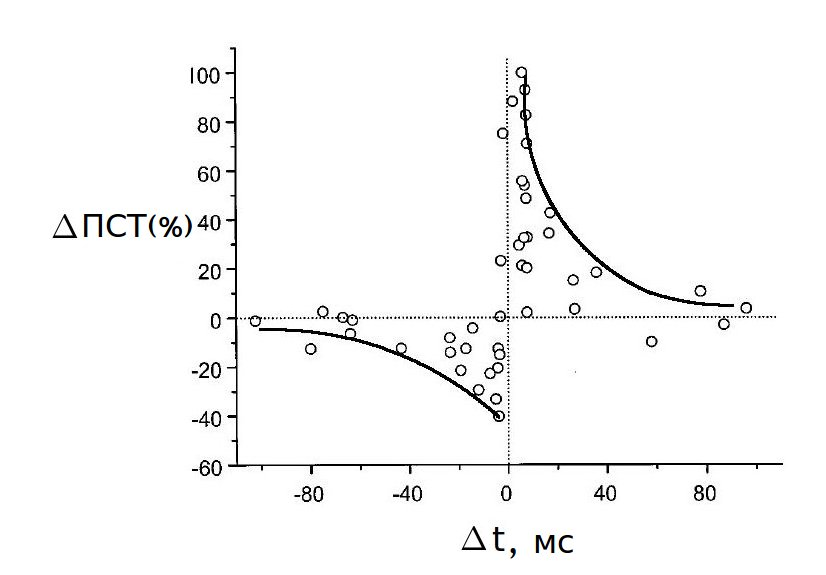
\includegraphics[width=75mm,scale=0.7]{stdp.jpg}
\caption{Спайко-временная пластичность. Зависимость $\Delta t = t_{post} - t_{pre}$ от изменения постсинаптического тока (ПСТ) на синапсе. Адаптировано из работы Г. Би и М. Пу \cite{stdp4}. }
\label{stdp_pic}
\end{figure}
\FloatBarrier
\indent Открытие этого феномена спровоцировало научное сообщество к новым дебатам на тему спайкового кода. С 1928-ого года, когда Э. Эдриан\cite{rate_first} предложил, что информация о стимуле хранится в спайковой активности усреднённой на относительно большом временном окне (100 мс), большинство нейрофизиологов на протяжении 20-ого века были на стороне данной гипотезы. В конце 20-ого века, мнения разделилсь, что послужило катализатором для новых исследований.\\
\subsubsection{Теория БКМ (BCM theory)}
\indent Теория БКМ, названная инициалами фамилий трёх учёных разработавших её: Э. Бйаненшток, Л. Купер и П. Монро (E. Bienenstock, L.Cooper и P.Munro), это физическая теория описывающая обучение в зрительной коре. Данная теория знаменита своими предсказаниями, которые подтверждались неоднократно экспериментами \cite{Cooper}.\\
\indent Теория пластичности синапсов предлагаемая БКМ теорией имеет в своей основе теорию Хэбба, и, по сути, является ещё одной модифицикацией, которая решает проблему стабильности классического правила Хэбба.\\


\subsection{Обучение на основе феноменологической модели STDP}
\subsection{Теоретическая оптимальная модель STDP}
\section{Обучение с подкреплением}
\subsection{Трехфакторное правило обучения}
\subsection{Гедонистический синапс}
\subsection{Обучение на основе TD-ошибки}
\section{Выводы}
\section{Использованная литература}
\bibliography{refs}{}
\bibliographystyle{unsrt}

\end{document}
